\documentclass{beamer}
\usepackage{booktabs}
\usepackage{pdfpages}
\usepackage{mathtools}
\usepackage{enumerate}
\usepackage{multirow,tabularx}
\usepackage{booktabs}
\usepackage{pdfpages}
\usepackage{proof}
\usepackage{cancel}
\usepackage{chronology}
\usepackage{graphicx}
\usepackage{ulem}
\usepackage{amsmath}
\usepackage{amssymb}
\usepackage{color}
\usepackage{animate}
\usepackage{xr}

\PassOptionsToPackage{usenames,dvipsnames,svgnames}{xcolor}  
\usepackage{tikz}
\usepackage{tkz-graph}


\usepackage{wasysym}
\usepackage{proof}
\usepackage{cancel}
\usepackage{chronology}
\usepackage{graphicx}
\usepackage{ulem}
\usepackage{amsmath}
\usepackage{amssymb}
\usepackage{color}
\usepackage{xcolor}
\usepackage{soul}
%\usepackage{pstricks}
\setbeamertemplate{navigation symbols}{}

\newcommand{\norm}[1]{\left\lVert#1\right\rVert}
\newcommand{\el}{$\mathcal{EL}^{++}$}
\renewcommand{\Re}{\mathbb{R}}
\newcommand{\BigO}[1]{\ensuremath{\operatorname{O}\bigl(#1\bigr)}}
\newcommand{\myul}[2][blue]{\sethlcolor{#1}\hl{#2}\setulcolor{black}}

\newcommand<>{\cunderline}[3]{\only<#1>{#3}\only<#2>{\underline{#3}}}
\newcommand<>{\cem}[3]{\only<#1>{#3}\only<#2>{\ul{#3}}}
\newcommand<>{\cgray}[3]{\only<#1>{#3}\only<#2>{\textcolor{gray}{#3}}}
\newcommand<>{\colorize}[4]{\only<#1>{#4}\only<#2>{\textcolor{#3}{#4}}}

\setbeamertemplate{navigation symbols}{\insertslidenavigationsymbol}
%\setbeamertemplate{navigation symbols}{}
% \addtobeamertemplate{navigation symbols}{}{%
%     \usebeamerfont{footline}%
%     \usebeamercolor[fg]{footline}%
%     \hspace{1em}%
%     \insertframenumber/\inserttotalframenumber
% }

\mode<presentation>
{
\usecolortheme{crane}
%\useoutertheme{split}

\expandafter\def\expandafter\insertshorttitle\expandafter{%
  \insertshorttitle\hfill%
  \insertframenumber\,/\,\inserttotalframenumber}

\usefonttheme[onlysmall]{structurebold}
}
\renewcommand{\em}{\itshape}
\usepackage{pifont}
\definecolor{purple}{rgb}{1,0,1}
\definecolor{dred}{rgb}{0.7,0,0}
\definecolor{myred}{rgb}{1,0,0}
\definecolor{dblue}{rgb}{0,0,0.7}
\definecolor{dgreen}{rgb}{0,0.5,0}
\definecolor{myyellow}{rgb}{1,1,0}
\newcommand{\parents}[1]{parents(#1)}
\setbeamertemplate{itemize item}[ball]


% \mode<presentation>
% {
% \useinnertheme[shadow=true]{rounded}
% \useoutertheme{infolines}
% \usecolortheme{dove}
% \setbeamerfont{block title}{size={}}
% }

\title[Bio-Ontologies]{Semantic similarity and machine learning with
  ontologies}
\subtitle{A brief introduction}

\author{Robert Hoehndorf}


\date{\url{https://github.com/bio-ontology-research-group/ontology-tutorial}}

\begin{document}

\begin{frame}
  \titlepage
\end{frame}

\begin{frame}
  \frametitle{Semantic similarity: some examples}
  \begin{itemize}
  \item Are cyclin dependent kinases {\em functionally} more similar
    to lipid kinases or to riboflavin kinases? How about {\em
      phenotypically}?
  \item Which protein in the {\em mouse} is functionally most similar
    to the zebrafish {\em gustducin} protein?
  \item Which mouse knockout resembles {\em Bardet-Biedl Syndrome 8}?
  \item Are there mouse knockouts that resemble the side effects of
    diclofenac?
  \item Which genetic disease produces similar symptoms to ebola?
  \item Does functional similarity correlate with phenotypic
    similarity?
  \end{itemize}
\end{frame}

\begin{frame}
  \frametitle{Semantic similarity}
  semantic similarity measures:
  \begin{itemize}
  \item for words, terms, classes
  \item role of background knowledge:
    \begin{itemize}
    \item statistical/distributional semantics, large corpora
    \item ontologies: (graph) topology
    \end{itemize}
  \item similarity measures: hand-crafted or data-driven?
  \end{itemize}
\end{frame}

\begin{frame}
  \frametitle{Semantic similarity or machine learning}
  \begin{itemize}
  \item semantic similarity measures are mostly hand-crafted
    \begin{itemize}
    \item capture certain intuition about what constitutes
      ``similarity''
    \item different measures for different kinds of similarity
    \item usually interpretable (and explainable)
    \end{itemize}
    \pause
  \item machine learning methods are mostly data-driven
    \begin{itemize}
    \item the architecture of the model is still hand-crafted
    \item usually hard to interpret
    \end{itemize}
  \end{itemize}
\end{frame}

\begin{frame}
  \frametitle{Ontologies and graphs}
  \begin{itemize}
  \item semantic similarity measures {\em and machine learning models} on
    ontologies can be graph-based, feature-based, or model-based
    \begin{itemize}
    \item graph-based: ontology as a graph
    \item feature-based: extract (or obtain) features for
      classes/relations (e.g., from axioms)
    \item model-based: define similarity within (special) $\Sigma$-structures
    \end{itemize}
    \pause
  \item we may need to generate graphs from ontologies
    \begin{itemize}
    \item {\em is-a} relations are easy (this is just {\tt owl:subClassOf})
    \item how about {\em part-of}, {\em regulates}, {\em precedes},
      etc.?
    \item disjointness, universal vs. existential quantification,
      cardinality restrictions, intersection, union, negation?
    \end{itemize}
    \pause
  \item relational patterns are implicit in OWL axioms
    \begin{itemize}
    \item design patterns as ``relations'' between classes
    \end{itemize}
  \end{itemize}
\end{frame}

\begin{frame}
  \frametitle{Relations as patterns}
  \centerline{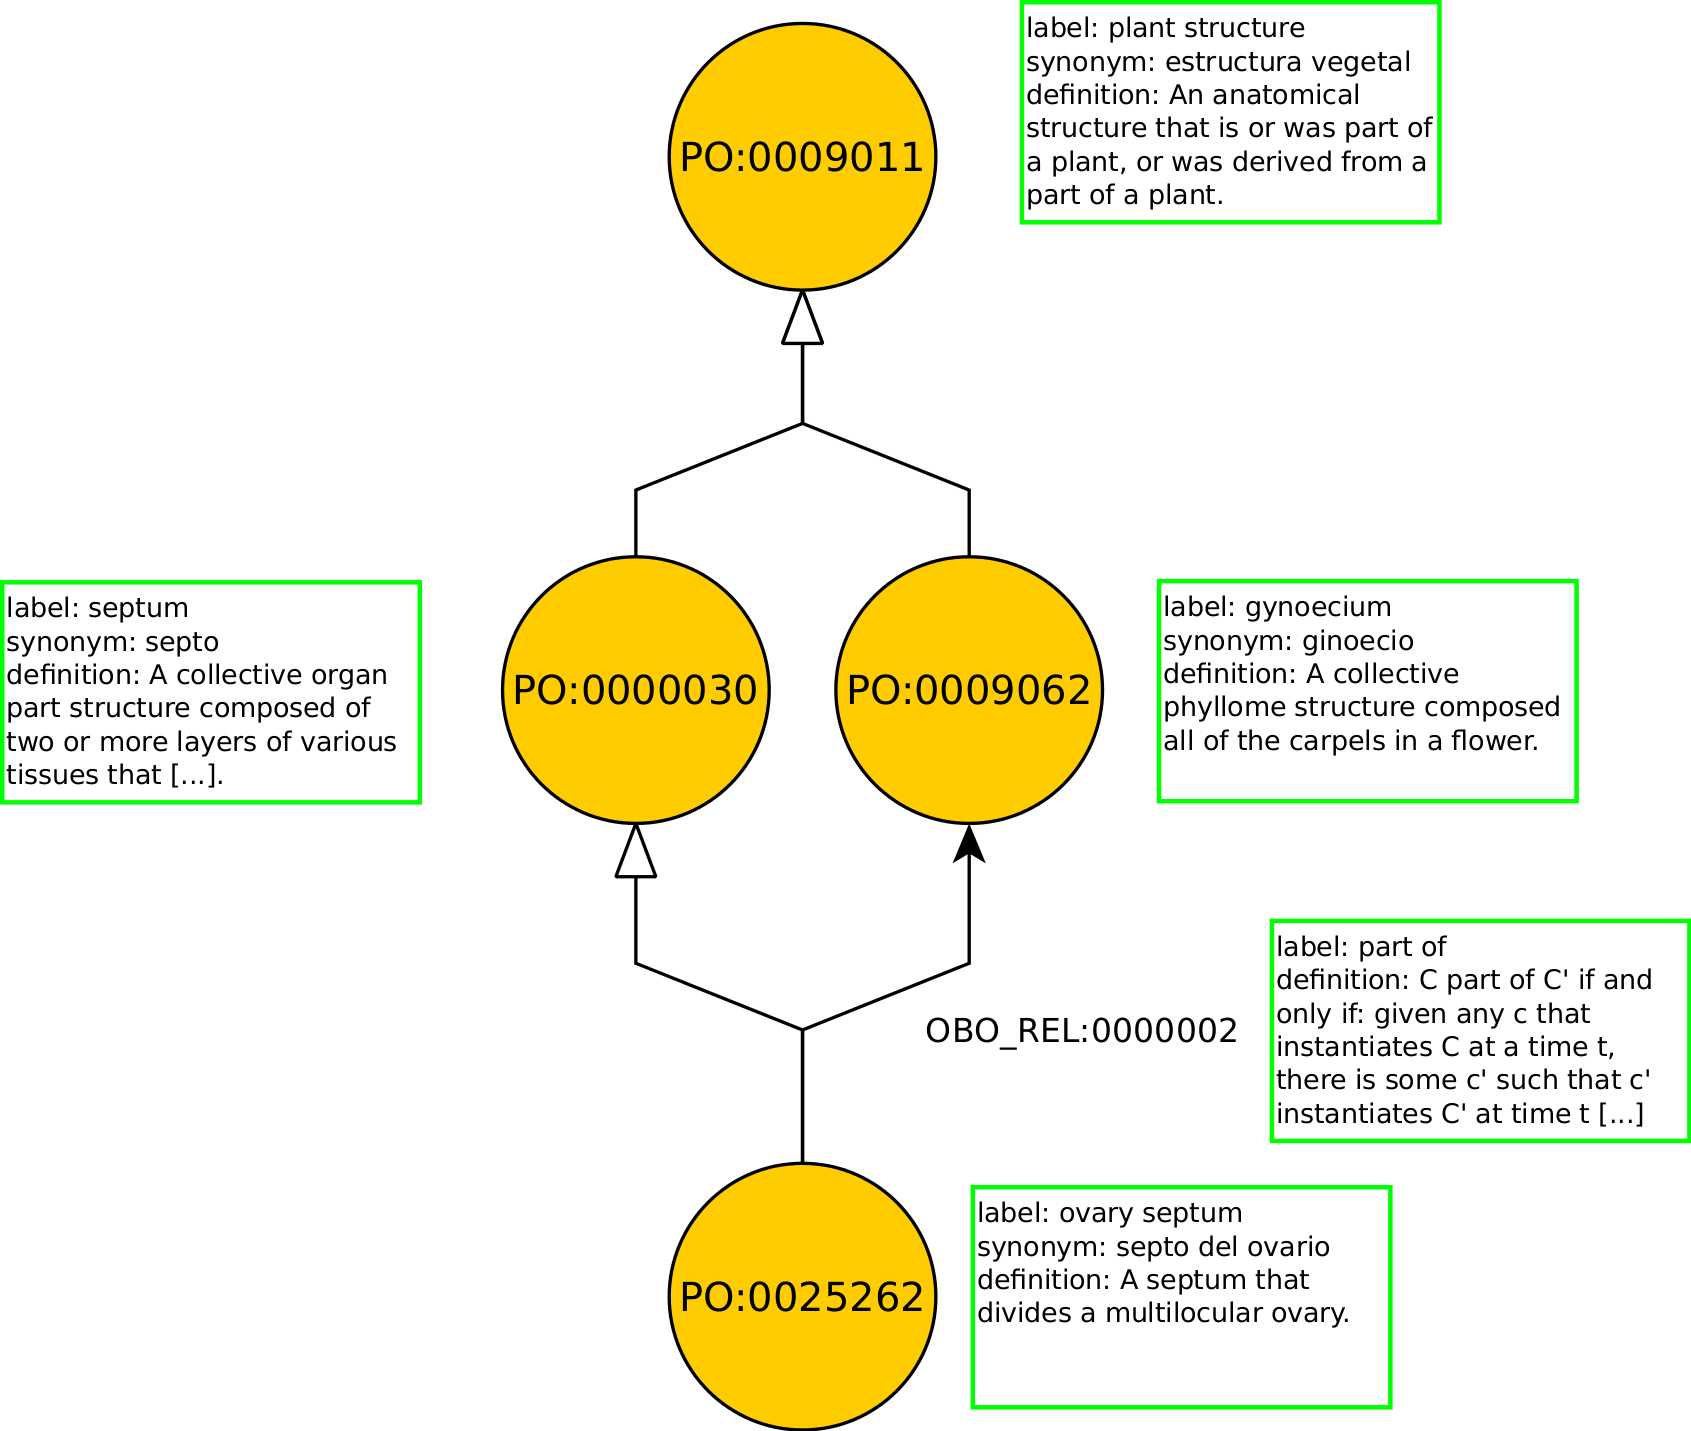
\includegraphics[height=.8\textheight]{plant-ontology-sample.png}}
\end{frame}

% \begin{frame}
%   \frametitle{Relations as patterns}
%   \begin{itemize}
%   \item OBO Relation Ontology (RO):
%     \begin{itemize}
%     \item \url{https://github.com/oborel/obo-relations}
%     \end{itemize}
%   \item Basic Formal Ontology (BFO):
%     \begin{itemize}
%     \item provides top-level classes
%       \begin{itemize}
%       \item Continuant, Process, Function, Material object, etc.
%       \end{itemize}
%     \item used for some OBO Foundry ontologies
%     \end{itemize}
%   \item RO and BFO provide a top-level system of classes and relations
%     shared across many biomedical ontologies
%   \item this system may define patterns used to generate graphs
%   \end{itemize}
% \end{frame}

\begin{frame}
  \frametitle{Relations as patterns}
  \begin{itemize}
  \item {\tt X SubClassOf: Y}: $X \xrightarrow{\text{is-a}} Y$
  \item {\tt X SubClassOf: part-of some Y}: $X \xrightarrow{\text{part-of}} Y$
  \item {\tt X SubClassOf: regulates some Y}: $X \xrightarrow{\text{regulates}} Y$
  \item {\tt X DisjointWith: Y}: $X \xleftrightarrow{\text{disjoint}} Y$
  \item {\tt X EquivalentTo: Y}: $X \xleftrightarrow{\equiv} Y$,
    $\{X,Y\}$
  \item ...
  \end{itemize}
  NB: in bio-ontologies, the OBO Relation Ontology defines these
  patterns
\end{frame}

\begin{frame}
  \frametitle{Asserted and inferred}
  \begin{itemize}
  \item relation patterns can be asserted or inferred
  \item {\tt X SubClassOf: part-of some Y}
  \item {\tt Y SubClassOf: part-of some Z}
  \item {\tt part-of o part-of SubPropertyOf: part-of}
  \item $\vdash$ {\tt X SubClassOf: part-of some Z}
  \item Therefore: $X \xrightarrow{\text{part-of}} Z$
  \item $\Rightarrow$ we should use deductive inference to generate
    these patterns
  \end{itemize}
\end{frame}

\section{Semantic similarity}

\begin{frame}
  Semantic similarity
  \begin{itemize}
  \item We want to use {\em  background knowledge} in ontologies to
    \begin{itemize}
    \item determine similarity between classes,
    \item instances,
    \item and entities with ontology annotations
    \end{itemize}
  \end{itemize}
\end{frame}


\begin{frame}
  \frametitle{How to measure similarity?}
  \begin{itemize}
  \item semantic similarity measures similarity between classes
  \item semantic similarity measures similarity between instances of classes
  \item semantic similarity measures similarity between entities
    {\em annotated} with classes
  \item $\Rightarrow$ reduce all of this to similarity between classes
  \end{itemize}
\end{frame}

\begin{frame}
  \frametitle{How to measure similarity?}
  What properties do we want in a similarity measure?
  \\
  A function $sim: D \times D$ is a similarity on $D$ if, for
  all $x, y \in D$, the function $sim$ is:  \begin{itemize}
    \pause
  \item non-negative: $sim(x,y) \geq 0$ for all $x, y$
    \pause
  \item symmetric: $sim(x,y) = sim(y,x)$
    \pause
  \item reflexive: $sim(x,x) = max_D$
    \pause
    \begin{itemize}
    \item weaker form: $sim(x,x) > sim(x,y)$ for all $x \not= y$
    \end{itemize}
    \pause
  \item $sim(x,x) > sim(x,y)$ for $x\not= y$
    \pause
  \item $sim$ is a {\em normalized} similarity measure if it has
    values in $[0,1]$
  \end{itemize}
\end{frame}

\usetikzlibrary{arrows,positioning,automata}
\begin{frame}
  \frametitle{How to measure similarity?}
  \begin{columns}
    \begin{column}{.6\textwidth}
      {\tiny
        \begin{tikzpicture}[>=stealth',shorten >=1pt,node distance=2cm,on grid,initial/.style    ={}]
          \node[state]          (A)                        {$Thing$};
          \node[state]          (B) [below left =of A]    {$Color$};
          \node[state]          (C) [below right =of A]    {$Shape$};
          \node[state]          (D) [below left =of B]    {$Red$};
          \node[state]          (H) [below right =of B]    {$Green$};
          \node[state]          (E) [below  =of D]    {$Orange$};
          \node[state]          (F) [below =of C]    {$Round$};
          \node[state]          (G) [below right =of C]    {$Square$};
          \tikzset{mystyle/.style={->,double=orange}} 
          \tikzset{every node/.style={fill=white}} 
          \path (B)     edge [mystyle]    node   {$isa$} (A)
          (C)     edge [mystyle]    node   {$isa$} (A) 
          (D)     edge [mystyle]    node   {$isa$} (B)
          (H)     edge [mystyle]    node   {$isa$} (B)
          (E)     edge [mystyle]    node   {$isa$} (D)
          (F)     edge [mystyle]    node   {$isa$} (C)
          (G)     edge [mystyle]    node   {$isa$} (C);
          \tikzset{mystyle/.style={<->,double=orange}}   
          \tikzset{mystyle/.style={<->,relative=true,in=0,out=60,double=orange}}
        \end{tikzpicture}
      }
    \end{column}
    \begin{column}{.4\textwidth}
      \begin{itemize}
        \pause
      \item distance on shortest path (Rada {\em et al.}, 1989)
        \pause
      \item $dist_{Rada}(u,v) = sp(u, isa, v)$
        \pause
      \item $sim_{Rada}(u,v) = \frac{1}{dist_{Rada}(u,v) + 1}$
      \end{itemize}
    \end{column}
  \end{columns}
\end{frame}

\begin{frame}
  \frametitle{How to measure similarity?}
  \begin{columns}
    \begin{column}{.6\textwidth}
      {\tiny
        \begin{tikzpicture}[>=stealth',shorten >=1pt,node distance=2cm,on grid,initial/.style    ={}]
          \node[state]          (A)                        {$Thing$};
          \node[state]          (B) [below left =of A]    {$Color$};
          \node[state]          (C) [below right =of A]    {$Shape$};
          \node[state, fill=green]          (D) [below left =of B]    {$Red$};
          \node[state, fill=green]          (H) [below right =of B]    {$Green$};
          \node[state]          (E) [below  =of D]    {$Orange$};
          \node[state]          (F) [below =of C]    {$Round$};
          \node[state]          (G) [below right =of C]    {$Square$};
          \tikzset{mystyle/.style={->,double=orange}} 
          \tikzset{highlight/.style={->,double=green}} 
          \tikzset{every node/.style={fill=white}}
          \path (B)     edge [mystyle]    node   {$isa$} (A)
          (C)     edge [mystyle]    node   {$isa$} (A) 
          (D)     edge [highlight]    node   {$isa$} (B)
          (H)     edge [highlight]    node   {$isa$} (B)
          (E)     edge [mystyle]    node   {$isa$} (D)
          (F)     edge [mystyle]    node   {$isa$} (C)
          (G)     edge [mystyle]    node   {$isa$} (C);
          \tikzset{mystyle/.style={<->,double=orange}}   
          \tikzset{mystyle/.style={<->,relative=true,in=0,out=60,double=orange}}
        \end{tikzpicture}
      }
    \end{column}
    \begin{column}{.4\textwidth}
      \begin{itemize}
      \item distance on shortest path
        \pause
       \item distance(green, red) = 2
       \item $sim_{Rada}(green, red) = \frac{1}{3}$
      \end{itemize}
    \end{column}
  \end{columns}
\end{frame}

\begin{frame}
  \frametitle{How to measure similarity?}
  \begin{columns}
    \begin{column}{.6\textwidth}
      {\tiny
        \begin{tikzpicture}[>=stealth',shorten >=1pt,node distance=2cm,on grid,initial/.style    ={}]
          \node[state]          (A)                        {$Thing$};
          \node[state]          (B) [below left =of A]    {$Color$};
          \node[state]          (C) [below right =of A]    {$Shape$};
          \node[state]          (D) [below left =of B]    {$Red$};
          \node[state]          (H) [below right =of B]    {$Green$};
          \node[state]          (E) [below  =of D]    {$Orange$};
          \node[state, fill=green]          (F) [below =of C]    {$Round$};
          \node[state, fill=green]          (G) [below right =of C]    {$Square$};
          \tikzset{mystyle/.style={->,double=orange}} 
          \tikzset{highlight/.style={->,double=green}} 
          \tikzset{every node/.style={fill=white}}
          \path (B)     edge [mystyle]    node   {$isa$} (A)
          (C)     edge [mystyle]    node   {$isa$} (A) 
          (D)     edge [mystyle]    node   {$isa$} (B)
          (H)     edge [mystyle]    node   {$isa$} (B)
          (E)     edge [mystyle]    node   {$isa$} (D)
          (F)     edge [highlight]    node   {$isa$} (C)
          (G)     edge [highlight]    node   {$isa$} (C);
          \tikzset{mystyle/.style={<->,double=orange}}   
          \tikzset{mystyle/.style={<->,relative=true,in=0,out=60,double=orange}}
        \end{tikzpicture}
      }
    \end{column}
    \begin{column}{.4\textwidth}
      \begin{itemize}
       \item distance on shortest path
       \item distance(square, round) = 2
       \item $sim_{Rada}(square, round) = \frac{1}{3}$
      \end{itemize}
    \end{column}
  \end{columns}
\end{frame}

\begin{frame}
  \frametitle{How to measure similarity?}
  \begin{columns}
    \begin{column}{.6\textwidth}
      {\tiny
        \begin{tikzpicture}[>=stealth',shorten >=1pt,node distance=2cm,on grid,initial/.style    ={}]
          \node[state]          (A)                        {$Thing$};
          \node[state, fill=green]          (B) [below left =of A]    {$Color$};
          \node[state]          (C) [below right =of A]    {$Shape$};
          \node[state]          (D) [below left =of B]    {$Red$};
          \node[state]          (H) [below right =of B]    {$Green$};
          \node[state, fill=green]          (E) [below  =of D]    {$Orange$};
          \node[state]          (F) [below =of C]    {$Round$};
          \node[state]          (G) [below right =of C]    {$Square$};
          \tikzset{mystyle/.style={->,double=orange}} 
          \tikzset{highlight/.style={->,double=green}} 
          \tikzset{every node/.style={fill=white}}
          \path (B)     edge [mystyle]    node   {$isa$} (A)
          (C)     edge [mystyle]    node   {$isa$} (A) 
          (D)     edge [highlight]    node   {$isa$} (B)
          (H)     edge [mystyle]    node   {$isa$} (B)
          (E)     edge [highlight]    node   {$isa$} (D)
          (F)     edge [mystyle]    node   {$isa$} (C)
          (G)     edge [mystyle]    node   {$isa$} (C);
          \tikzset{mystyle/.style={<->,double=orange}}   
          \tikzset{mystyle/.style={<->,relative=true,in=0,out=60,double=orange}}
        \end{tikzpicture}
      }
    \end{column}
    \begin{column}{.4\textwidth}
      \begin{itemize}
       \item distance on shortest path
       \item distance(orange, color) = 2
       \item $sim_{Rada}(orange, color) = \frac{1}{3}$
      \end{itemize}
    \end{column}
  \end{columns}
\end{frame}

\begin{frame}
  \frametitle{How to measure similarity?}
  \begin{itemize}
  \item shortest path is not always intuitive
    \pause
  \item we need a way to determine {\em specificity} of a class
    \begin{itemize}
    \item number of ancestors
    \item number of children
    \item information content
    \end{itemize}
    \pause
  \item {\em density} of a branch in the ontology
    \begin{itemize}
    \item number of siblings
    \item information content
    \end{itemize}
    \pause
  \item account for different edge types
    \begin{itemize}
    \item non-uniform edge weighting
    \end{itemize}
  \end{itemize}
\end{frame}

\begin{frame}
  \frametitle{How to measure similarity}
  \begin{itemize}
  \item term specificity measure $\sigma: C \mapsto \mathbb{R}$:
    \begin{itemize}
    \item $x \sqsubseteq y \rightarrow \sigma(x) \geq \sigma(y)$
    \end{itemize}
    \pause
  \item intrinsic:
    \begin{itemize}
    \item $\sigma(x) = f(depth(x))$
    \item $\sigma(x) = f(A(x))$ (for ancestors $A(x)$)
    \item $\sigma(x) = f(D(x))$ (for descendants $D(x)$)
    \item many more, e.g., Zhou et al.: $\sigma(x) = k \cdot \Big( 1-\frac{\log
        |D(x)|}{\log |C|} \Big) + (1-k) \frac{\log depth(x)}{\log
        depth(G_T)} $
    \end{itemize}
    \pause
  \item extrinsic:
    \begin{itemize}
    \item $\sigma(x)$ defined as a function of instances (or annotations) $I$
      \begin{itemize}
      \item note: the number of instances monotonically decreases with
        increasing depth in taxonomies
      \end{itemize}
    \item Resnik 1995: $eIC_{Resnik}(x) = -\log p(x)$ (with $p(x) =
      \frac{|I(x)|}{|I|}$)
      \begin{itemize}
      \item in biology, one of the most popular specificity measure when
        annotations are present
      \end{itemize}
    \end{itemize}
  \end{itemize}
\end{frame}

\begin{frame}
  \frametitle{How to measure similarity?}
  \begin{columns}
    \begin{column}{.6\textwidth}
      {\tiny
        \begin{tikzpicture}[>=stealth',shorten >=1pt,node distance=2cm,on grid,initial/.style    ={}]
          \node[state,label=below:$0.0$]          (A)                        {$Thing$};
          \node[state,label=below:$1.0$]          (B) [below left =of A]    {$Color$};
          \node[state,label=right:$1.0$]          (C) [below right =of A]    {$Shape$};
          \node[state,label=right:$2.0$]          (D) [below left =of B]    {$Red$};
          \node[state,label=below:$2.0$]          (H) [below right =of B]    {$Green$};
          \node[state,label=below:$3.0$]          (E) [below  =of D]    {$Orange$};
          \node[state,label=below:$2.0$]          (F) [below =of C]    {$Round$};
          \node[state,label=below:$2.0$]          (G) [below right =of C]    {$Square$};
          \tikzset{mystyle/.style={->,double=orange}} 
          \tikzset{highlight/.style={->,double=green}} 
          \tikzset{every node/.style={fill=white}}
          \path (B)     edge [mystyle]    node   {$isa$} (A)
          (C)     edge [mystyle]    node   {$isa$} (A) 
          (D)     edge [mystyle]    node   {$isa$} (B)
          (H)     edge [mystyle]    node   {$isa$} (B)
          (E)     edge [mystyle]    node   {$isa$} (D)
          (F)     edge [mystyle]    node   {$isa$} (C)
          (G)     edge [mystyle]    node   {$isa$} (C);
          \tikzset{mystyle/.style={<->,double=orange}}   
          \tikzset{mystyle/.style={<->,relative=true,in=0,out=60,double=orange}}
        \end{tikzpicture}
      }
    \end{column}
    \begin{column}{.4\textwidth}
      \begin{itemize}
      \item Resnik 1995: similarity between $x$ and $y$ is the
        information content of the {\em most informative common
          ancestor}
      \end{itemize}
    \end{column}
  \end{columns}
\end{frame}

\begin{frame}
  \frametitle{How to measure similarity?}
  \begin{columns}
    \begin{column}{.6\textwidth}
      {\tiny
        \begin{tikzpicture}[>=stealth',shorten >=1pt,node distance=2cm,on grid,initial/.style    ={}]
          \node[state,label=below:$0.0$]          (A)                        {$Thing$};
          \node[state,label=below:$1.0$]          (B) [below left =of A]    {$Color$};
          \node[state,label=right:$1.0$]          (C) [below right =of A]    {$Shape$};
          \node[state,fill=green,label=right:$2.0$]          (D) [below left =of B]    {$Red$};
          \node[state,fill=green,label=below:$2.0$]          (H) [below right =of B]    {$Green$};
          \node[state,label=below:$3.0$]          (E) [below  =of D]    {$Orange$};
          \node[state,label=below:$2.0$]          (F) [below =of C]    {$Round$};
          \node[state,label=below:$2.0$]          (G) [below right =of C]    {$Square$};
          \tikzset{mystyle/.style={->,double=orange}} 
          \tikzset{highlight/.style={->,double=green}} 
          \tikzset{every node/.style={fill=white}}
          \path (B)     edge [mystyle]    node   {$isa$} (A)
          (C)     edge [mystyle]    node   {$isa$} (A) 
          (D)     edge [mystyle]    node   {$isa$} (B)
          (H)     edge [mystyle]    node   {$isa$} (B)
          (E)     edge [mystyle]    node   {$isa$} (D)
          (F)     edge [mystyle]    node   {$isa$} (C)
          (G)     edge [mystyle]    node   {$isa$} (C);
          \tikzset{mystyle/.style={<->,double=orange}}   
          \tikzset{mystyle/.style={<->,relative=true,in=0,out=60,double=orange}}
        \end{tikzpicture}
      }
    \end{column}
    \begin{column}{.4\textwidth}
      \begin{itemize}
      \item Resnik 1995: similarity between $x$ and $y$ is the
        information content of the {\em most informative common
          ancestor}
      \end{itemize}
    \end{column}
  \end{columns}
\end{frame}

\begin{frame}
  \frametitle{How to measure similarity?}
  \begin{columns}
    \begin{column}{.6\textwidth}
      {\tiny
        \begin{tikzpicture}[>=stealth',shorten >=1pt,node distance=2cm,on grid,initial/.style    ={}]
          \node[state,label=below:$0.0$]          (A)                        {$Thing$};
          \node[state,fill=yellow,label=below:$1.0$]          (B) [below left =of A]    {$Color$};
          \node[state,label=right:$1.0$]          (C) [below right =of A]    {$Shape$};
          \node[state,fill=green,label=right:$2.0$]          (D) [below left =of B]    {$Red$};
          \node[state,fill=green,label=below:$2.0$]          (H) [below right =of B]    {$Green$};
          \node[state,label=below:$3.0$]          (E) [below  =of D]    {$Orange$};
          \node[state,label=below:$2.0$]          (F) [below =of C]    {$Round$};
          \node[state,label=below:$2.0$]          (G) [below right =of C]    {$Square$};
          \tikzset{mystyle/.style={->,double=orange}} 
          \tikzset{highlight/.style={->,double=green}} 
          \tikzset{every node/.style={fill=white}}
          \path (B)     edge [mystyle]    node   {$isa$} (A)
          (C)     edge [mystyle]    node   {$isa$} (A) 
          (D)     edge [mystyle]    node   {$isa$} (B)
          (H)     edge [mystyle]    node   {$isa$} (B)
          (E)     edge [mystyle]    node   {$isa$} (D)
          (F)     edge [mystyle]    node   {$isa$} (C)
          (G)     edge [mystyle]    node   {$isa$} (C);
          \tikzset{mystyle/.style={<->,double=orange}}   
          \tikzset{mystyle/.style={<->,relative=true,in=0,out=60,double=orange}}
        \end{tikzpicture}
      }
    \end{column}
    \begin{column}{.4\textwidth}
      \begin{itemize}
      \item Resnik 1995: similarity between $x$ and $y$ is the
        information content of the {\em most informative common
          ancestor}
      \end{itemize}
    \end{column}
  \end{columns}
\end{frame}

\begin{frame}
  \frametitle{How to measure similarity?}
  \begin{columns}
    \begin{column}{.6\textwidth}
      {\tiny
        \begin{tikzpicture}[>=stealth',shorten >=1pt,node distance=2cm,on grid,initial/.style    ={}]
          \node[state,label=below:$0.0$]          (A)                        {$Thing$};
          \node[state,fill=yellow,label=below:$1.0$]          (B) [below left =of A]    {$Color$};
          \node[state,label=right:$1.0$]          (C) [below right =of A]    {$Shape$};
          \node[state,fill=green,label=right:$2.0$]          (D) [below left =of B]    {$Red$};
          \node[state,fill=green,label=below:$2.0$]          (H) [below right =of B]    {$Green$};
          \node[state,label=below:$3.0$]          (E) [below  =of D]    {$Orange$};
          \node[state,label=below:$2.0$]          (F) [below =of C]    {$Round$};
          \node[state,label=below:$2.0$]          (G) [below right =of C]    {$Square$};
          \tikzset{mystyle/.style={->,double=orange}} 
          \tikzset{highlight/.style={->,double=green}} 
          \tikzset{every node/.style={fill=white}}
          \path (B)     edge [mystyle]    node   {$isa$} (A)
          (C)     edge [mystyle]    node   {$isa$} (A) 
          (D)     edge [mystyle]    node   {$isa$} (B)
          (H)     edge [mystyle]    node   {$isa$} (B)
          (E)     edge [mystyle]    node   {$isa$} (D)
          (F)     edge [mystyle]    node   {$isa$} (C)
          (G)     edge [mystyle]    node   {$isa$} (C);
          \tikzset{mystyle/.style={<->,double=orange}}   
          \tikzset{mystyle/.style={<->,relative=true,in=0,out=60,double=orange}}
        \end{tikzpicture}
      }
    \end{column}
    \begin{column}{.4\textwidth}
      \begin{itemize}
      \item Resnik 1995: similarity between $x$ and $y$ is the
        information content of the {\em most informative common
          ancestor}
        \item $sim_{Resnik}(Green, Red) = 1.0$
      \end{itemize}
    \end{column}
  \end{columns}
\end{frame}

\begin{frame}
  \frametitle{How to measure similarity?}
  \begin{columns}
    \begin{column}{.6\textwidth}
      {\tiny
        \begin{tikzpicture}[>=stealth',shorten >=1pt,node distance=2cm,on grid,initial/.style    ={}]
          \node[state,label=below:$0.0$]          (A)                        {$Thing$};
          \node[state,fill=yellow,label=below:$1.0$]          (B) [below left =of A]    {$Color$};
          \node[state,label=right:$1.0$]          (C) [below right =of A]    {$Shape$};
          \node[state,label=right:$2.0$]          (D) [below left =of B]    {$Red$};
          \node[state,fill=green,label=below:$2.0$]          (H) [below right =of B]    {$Green$};
          \node[state,fill=green,label=below:$3.0$]          (E) [below  =of D]    {$Orange$};
          \node[state,label=below:$2.0$]          (F) [below =of C]    {$Round$};
          \node[state,label=below:$2.0$]          (G) [below right =of C]    {$Square$};
          \tikzset{mystyle/.style={->,double=orange}} 
          \tikzset{highlight/.style={->,double=green}} 
          \tikzset{every node/.style={fill=white}}
          \path (B)     edge [mystyle]    node   {$isa$} (A)
          (C)     edge [mystyle]    node   {$isa$} (A) 
          (D)     edge [mystyle]    node   {$isa$} (B)
          (H)     edge [mystyle]    node   {$isa$} (B)
          (E)     edge [mystyle]    node   {$isa$} (D)
          (F)     edge [mystyle]    node   {$isa$} (C)
          (G)     edge [mystyle]    node   {$isa$} (C);
          \tikzset{mystyle/.style={<->,double=orange}}   
          \tikzset{mystyle/.style={<->,relative=true,in=0,out=60,double=orange}}
        \end{tikzpicture}
      }
    \end{column}
    \begin{column}{.4\textwidth}
      \begin{itemize}
      \item Resnik 1995: similarity between $x$ and $y$ is the
        information content of the {\em most informative common
          ancestor}
        \item $sim_{Resnik}(Green, Orange) = 1.0$
      \end{itemize}
    \end{column}
  \end{columns}
\end{frame}

\begin{frame}
  \frametitle{How to measure similarity?}
  \begin{columns}
    \begin{column}{.6\textwidth}
      {\tiny
        \begin{tikzpicture}[>=stealth',shorten >=1pt,node distance=2cm,on grid,initial/.style    ={}]
          \node[state,fill=yellow,label=below:$0.0$]          (A)                        {$Thing$};
          \node[state,label=below:$1.0$]          (B) [below left =of A]    {$Color$};
          \node[state,label=right:$1.0$]          (C) [below right =of A]    {$Shape$};
          \node[state,label=right:$2.0$]          (D) [below left =of B]    {$Red$};
          \node[state,fill=green,label=below:$2.0$]          (H) [below right =of B]    {$Green$};
          \node[state,label=below:$3.0$]          (E) [below  =of D]    {$Orange$};
          \node[state,label=below:$2.0$]          (F) [below =of C]    {$Round$};
          \node[state,fill=green,label=below:$2.0$]          (G) [below right =of C]    {$Square$};
          \tikzset{mystyle/.style={->,double=orange}} 
          \tikzset{highlight/.style={->,double=green}} 
          \tikzset{every node/.style={fill=white}}
          \path (B)     edge [mystyle]    node   {$isa$} (A)
          (C)     edge [mystyle]    node   {$isa$} (A) 
          (D)     edge [mystyle]    node   {$isa$} (B)
          (H)     edge [mystyle]    node   {$isa$} (B)
          (E)     edge [mystyle]    node   {$isa$} (D)
          (F)     edge [mystyle]    node   {$isa$} (C)
          (G)     edge [mystyle]    node   {$isa$} (C);
          \tikzset{mystyle/.style={<->,double=orange}}   
          \tikzset{mystyle/.style={<->,relative=true,in=0,out=60,double=orange}}
        \end{tikzpicture}
      }
    \end{column}
    \begin{column}{.4\textwidth}
      \begin{itemize}
      \item Resnik 1995: similarity between $x$ and $y$ is the
        information content of the {\em most informative common
          ancestor}
        \item $sim_{Resnik}(Square, Orange) = 0.0$
      \end{itemize}
    \end{column}
  \end{columns}
\end{frame}

\begin{frame}
  \frametitle{How to measure similarity?}
  \begin{itemize}
  \item (Red, Green) and (Orange, Green) have the same similarity
  \item need to incorporate the specificity of the compared classes
  \end{itemize}
\end{frame}

\begin{frame}
  \frametitle{How to measure similarity?}
  \begin{columns}
    \begin{column}{.6\textwidth}
      {\tiny
        \begin{tikzpicture}[>=stealth',shorten >=1pt,node distance=2cm,on grid,initial/.style    ={}]
          \node[state,label=below:$0.0$]          (A)                        {$Thing$};
          \node[state,fill=yellow,label=below:$1.0$]          (B) [below left =of A]    {$Color$};
          \node[state,label=right:$1.0$]          (C) [below right =of A]    {$Shape$};
          \node[state,fill=green,label=right:$2.0$]          (D) [below left =of B]    {$Red$};
          \node[state,fill=green,label=below:$2.0$]          (H) [below right =of B]    {$Green$};
          \node[state,label=below:$3.0$]          (E) [below  =of D]    {$Orange$};
          \node[state,label=below:$2.0$]          (F) [below =of C]    {$Round$};
          \node[state,label=below:$2.0$]          (G) [below right =of C]    {$Square$};
          \tikzset{mystyle/.style={->,double=orange}} 
          \tikzset{highlight/.style={->,double=green}} 
          \tikzset{every node/.style={fill=white}}
          \path (B)     edge [mystyle]    node   {$isa$} (A)
          (C)     edge [mystyle]    node   {$isa$} (A) 
          (D)     edge [mystyle]    node   {$isa$} (B)
          (H)     edge [mystyle]    node   {$isa$} (B)
          (E)     edge [mystyle]    node   {$isa$} (D)
          (F)     edge [mystyle]    node   {$isa$} (C)
          (G)     edge [mystyle]    node   {$isa$} (C);
          \tikzset{mystyle/.style={<->,double=orange}}   
          \tikzset{mystyle/.style={<->,relative=true,in=0,out=60,double=orange}}
        \end{tikzpicture}
      }
    \end{column}
    \begin{column}{.4\textwidth}
      \begin{itemize}
      \item Lin 1998: $sim_{Lin}(x,y) = \frac{2\cdot
          IC(MICA(x,y))}{IC(x) + IC(y)}$
        \pause
      \item $sim_{Lin}(Green, Red) = 0.5$
      \end{itemize}
    \end{column}
  \end{columns}
\end{frame}

\begin{frame}
  \frametitle{How to measure similarity?}
  \begin{columns}
    \begin{column}{.6\textwidth}
      {\tiny
        \begin{tikzpicture}[>=stealth',shorten >=1pt,node distance=2cm,on grid,initial/.style    ={}]
          \node[state,label=below:$0.0$]          (A)                        {$Thing$};
          \node[state,fill=yellow,label=below:$1.0$]          (B) [below left =of A]    {$Color$};
          \node[state,label=right:$1.0$]          (C) [below right =of A]    {$Shape$};
          \node[state,label=right:$2.0$]          (D) [below left =of B]    {$Red$};
          \node[state,fill=green,label=below:$2.0$]          (H) [below right =of B]    {$Green$};
          \node[state,fill=green,label=below:$3.0$]          (E) [below  =of D]    {$Orange$};
          \node[state,label=below:$2.0$]          (F) [below =of C]    {$Round$};
          \node[state,label=below:$2.0$]          (G) [below right =of C]    {$Square$};
          \tikzset{mystyle/.style={->,double=orange}} 
          \tikzset{highlight/.style={->,double=green}} 
          \tikzset{every node/.style={fill=white}}
          \path (B)     edge [mystyle]    node   {$isa$} (A)
          (C)     edge [mystyle]    node   {$isa$} (A) 
          (D)     edge [mystyle]    node   {$isa$} (B)
          (H)     edge [mystyle]    node   {$isa$} (B)
          (E)     edge [mystyle]    node   {$isa$} (D)
          (F)     edge [mystyle]    node   {$isa$} (C)
          (G)     edge [mystyle]    node   {$isa$} (C);
          \tikzset{mystyle/.style={<->,double=orange}}   
          \tikzset{mystyle/.style={<->,relative=true,in=0,out=60,double=orange}}
        \end{tikzpicture}
      }
    \end{column}
    \begin{column}{.4\textwidth}
      \begin{itemize}
      \item Lin 1998: $sim_{Lin}(x,y) = \frac{2\cdot
          IC(MICA(x,y))}{IC(x) + IC(y)}$
      \item $sim_{Lin}(Green, Orange) = 0.4$
      \end{itemize}
    \end{column}
  \end{columns}
\end{frame}

\begin{frame}
  \frametitle{How to measure similarity?}
  \begin{itemize}
  \item many(!) others:
    \begin{itemize}
    \item Jiang \& Conrath 1997
    \item Mazandu \& Mulder 2013
    \item Schlicker et al. 2009
    \item ...
  \end{itemize}
  \end{itemize}
\end{frame}

\begin{frame}
  \frametitle{How to measure similarity?}
  \begin{itemize}
  \item we only looked at comparing pairs of classes
  \item mostly, we want to compare {\em sets} of classes
    \begin{itemize}
    \item set of GO annotations
    \item set of signs and symptoms
    \item set of phenotypes
    \end{itemize}
  \item two approaches:
    \begin{itemize}
    \item compare each class individually, then merge
    \item directly set-based similarity measures
    \end{itemize}
  \end{itemize}
\end{frame}

\begin{frame}
  \frametitle{How to measure similarity?}
  \begin{columns}
    \begin{column}{.6\textwidth}
      {\tiny
        \begin{tikzpicture}[>=stealth',shorten >=1pt,node distance=2cm,on grid,initial/.style    ={}]
          \node[state,label=below:$0.0$]          (A)                        {$Thing$};
          \node[state,label=below:$1.0$]          (B) [below left =of A]    {$Color$};
          \node[state,label=right:$1.0$]          (C) [below right =of A]    {$Shape$};
          \node[state,fill=gray,label=right:$2.0$]          (D) [below left =of B]    {$Red$};
          \node[state,label=below:$2.0$]          (H) [below right =of B]    {$Green$};
          \node[state,fill=green,label=below:$3.0$]          (E) [below  =of D]    {$Orange$};
          \node[state,fill=gray,label=below:$2.0$]          (F) [below =of C]    {$Round$};
          \node[state,fill=green,label=below:$2.0$]          (G) [below right =of C]    {$Square$};
          \tikzset{mystyle/.style={->,double=orange}} 
          \tikzset{highlight/.style={->,double=green}} 
          \tikzset{every node/.style={fill=white}}
          \path (B)     edge [mystyle]    node   {$isa$} (A)
          (C)     edge [mystyle]    node   {$isa$} (A) 
          (D)     edge [mystyle]    node   {$isa$} (B)
          (H)     edge [mystyle]    node   {$isa$} (B)
          (E)     edge [mystyle]    node   {$isa$} (D)
          (F)     edge [mystyle]    node   {$isa$} (C)
          (G)     edge [mystyle]    node   {$isa$} (C);
          \tikzset{mystyle/.style={<->,double=orange}}   
          \tikzset{mystyle/.style={<->,relative=true,in=0,out=60,double=orange}}
        \end{tikzpicture}
      }
    \end{column}
    \begin{column}{.4\textwidth}
      \begin{itemize}
      \item similarity between a square-and-orange thing and a
        round-and-red thing
        \pause
      \item Pesquita et al., 2007:
        $simGIC(X,Y) = \frac{\sum_{c \in A(X) \cap A(Y)}
          IC(c)}{\sum_{c \in A(X) \cup A(Y)} IC(c)}$
      \end{itemize}
    \end{column}
  \end{columns}
\end{frame}

\begin{frame}
  \frametitle{How to measure similarity?}
  \begin{columns}
    \begin{column}{.6\textwidth}
      {\tiny
        \begin{tikzpicture}[>=stealth',shorten >=1pt,node distance=2cm,on grid,initial/.style    ={}]
          \node[state,fill=pink,label=below:$0.0$]          (A)                        {$Thing$};
          \node[state,fill=pink,label=below:$1.0$]          (B) [below left =of A]    {$Color$};
          \node[state,fill=pink,label=right:$1.0$]          (C) [below right =of A]    {$Shape$};
          \node[state,fill=gray,label=right:$2.0$]          (D) [below left =of B]    {$Red$};
          \node[state,label=below:$2.0$]          (H) [below right =of B]    {$Green$};
          \node[state,fill=green,label=below:$3.0$]          (E) [below  =of D]    {$Orange$};
          \node[state,fill=gray,label=below:$2.0$]          (F) [below =of C]    {$Round$};
          \node[state,fill=green,label=below:$2.0$]          (G) [below right =of C]    {$Square$};
          \tikzset{mystyle/.style={->,double=orange}} 
          \tikzset{highlight/.style={->,double=green}} 
          \tikzset{every node/.style={fill=white}}
          \path (B)     edge [mystyle]    node   {$isa$} (A)
          (C)     edge [mystyle]    node   {$isa$} (A) 
          (D)     edge [mystyle]    node   {$isa$} (B)
          (H)     edge [mystyle]    node   {$isa$} (B)
          (E)     edge [mystyle]    node   {$isa$} (D)
          (F)     edge [mystyle]    node   {$isa$} (C)
          (G)     edge [mystyle]    node   {$isa$} (C);
          \tikzset{mystyle/.style={<->,double=orange}}   
          \tikzset{mystyle/.style={<->,relative=true,in=0,out=60,double=orange}}
        \end{tikzpicture}
      }
    \end{column}
    \begin{column}{.4\textwidth}
      \begin{itemize}
      \item similarity between a square-and-orange thing and a
        round-and-red thing
      \item Pesquita et al., 2007:
        $simGIC(X,Y) = \frac{\sum_{c \in A(X) \cap A(Y)}
          IC(c)}{\sum_{c \in A(X) \cup A(Y)} IC(c)}$
      \item $simGIC(so,rr) = \frac{2}{11}$
      \end{itemize}
    \end{column}
  \end{columns}
\end{frame}

\begin{frame}
  \frametitle{How to measure similarity?}
  \begin{itemize}
  \item alternatively: use different merging strategies
  \item common: average, maximum, {\bf best-matching average}
    \begin{itemize}
    \item Average: $sim_A(X,Y) = \frac{\sum_{x\in X} \sum_{y \in Y} sim(x,y)}{|X| \times |Y|}$
    \item Max average: $sim_{MA}(X,Y) = \frac{1}{|X|} \sum_{x\in X} \max_{y \in Y} sim(x,y)$
    \item Best match average: $sim_{BMA}(X,Y) = \frac{sim_{MA}(X,Y) + sim_{MA}(Y,X)}{2}$
    \end{itemize}
  \end{itemize}
\end{frame}

\begin{frame}
  \frametitle{How to measure similarity?}
  \begin{itemize}
  \item Semantic Measures Library:
    \begin{itemize}
    \item comprehensive Java library
    \item \url{http://www.semantic-measures-library.org/}
    \end{itemize}
  \item R packages: GOSim, GOSemSim, HPOSim, LSAfun,
    ontologySimilarity,...
  \item Python: sematch, fastsemsim (GO only)
  \end{itemize}
\end{frame}

\begin{frame}
  \frametitle{Applications of semantic similarity}
  \begin{itemize}
  \item no obvious choice of similarity measure
  \item depends on application
    \begin{itemize}
    \item e.g., predicting PPIs in different organisms through
      similarity may benefit from a different similarity measure!
    \end{itemize}
  \item different similarity measures may react differently to biases
    in data
  \item needs some testing and experience
  \end{itemize}
\end{frame}

\begin{frame}
  \frametitle{Applications of semantic similarity}
  Recommendations:
  \begin{itemize}
  \item use Resnik's information content measure
  \item use Resnik's similarity
  \item use Best Match Average
  \item use the full ontology
  \item classify your ontology using an automated reasoner before
    applying semantic similarity
    \begin{itemize}
    \item although many ontologies come pre-classified
    \end{itemize}
  \item $\Rightarrow$ but there are many exceptions
    \begin{itemize}
    \item similar location $\Rightarrow$ use location subset of GO
    \item developmental phenotypes $\Rightarrow$ use developmental
      branch of phenotype ontology
    \end{itemize}
  \end{itemize}
\end{frame}

\begin{frame}
  \frametitle{Analyzing phenotypes}
  \framesubtitle{4,000 genetic diseases in OMIM, 6,000 in OrphaNet,
    have an unknown molecular basis}
  \centerline{\includegraphics[width=.5\textwidth]{omim-s.png}}
  \centerline{\includegraphics[width=1\textwidth]{omim_highlight.png}}
  \centerline{\includegraphics[width=.5\textwidth]{orphanet-logo.png}}
\end{frame}

\begin{frame}
  \frametitle{Analyzing phenotypes}
  \framesubtitle{Semantic similarity over phenotype ontologies
    measures phenotypic similarity}
  \begin{itemize}
  \item semantic similarity: similarity measure based on information
    contained in the axioms/structure of an ontology
    \begin{itemize}
    \item anatomy: front limb -- hind limb vs. front limb -- eye
    \item function: detection of salty taste -- detection of sweet
      taste vs. detection of salty taste -- apoptosis
    \item quality: red -- orange vs. red -- green vs. red -- round
    \end{itemize}
  \item $\Rightarrow$ phenotypic similarity combines similarity between anatomy,
    function, and quality
  \end{itemize}
\end{frame}

\begin{frame}
  \frametitle{Analyzing phenotypes}
  \centerline{\includegraphics[width=.8\textwidth]{model-human-obesity-slide.pdf}}
\end{frame}


\begin{frame}
  \frametitle{Analyzing phenotypes}
  \begin{columns}
    \begin{column}{7cm}
      \centerline{\includegraphics[width=0.9\textwidth]{roc-omim-mgi-1.png}}
    \end{column}
    \begin{column}{4cm}
      \begin{itemize}
      \item AUC (OMIM): 0.82
      \item AUC (MGI): 0.90
      \end{itemize}
    \end{column}
  \end{columns}
\end{frame}

\begin{frame}
  \frametitle{Bassoe Syndrome} 
  \framesubtitle{Signs and symptoms}
  \begin{itemize}
  \item skeletal:
    \begin{itemize}
    \item kyphosis, hypertensible joints, cubitus valgus
    \end{itemize}
  \item muscular:
    \begin{itemize}
    \item hypotonia, muscle hypotrophy, amyotrophy
    \end{itemize}
  \item behavior:
    \begin{itemize}
    \item abnormal gait, amimia
    \end{itemize}
  \item visual:
    \begin{itemize}
    \item cataract, strabismus
    \end{itemize}
  \item reproductive:
    \begin{itemize}
    \item hypogonadism, hypogenitalism, abnormal ovaries, hypoplastic
      testis, reduced fertility
    \end{itemize}
  \end{itemize}
\end{frame}

\begin{frame}
  \frametitle{Bassoe Syndrome} 
  \framesubtitle{HIP1 mouse phenotypes}
  {\small
  \begin{columns}
    \begin{column}{.4\textwidth}
      Bassoe Syndrome:
      \begin{itemize}
      \item kyphosis, hypertensible joints, cubitus valgus
      \item amyotrophy, hypotonia, muscle hypotrophy
      \item abnormal gait, amimia
      \item cataract, strabismus
      \item testicular atrophy, hypogonadism, hypogenitalism, abnormal
        ovaries, reduced fertility
      \end{itemize}
    \end{column}
    \begin{column}{.6\textwidth}
      Mouse phenotypes:
      \begin{itemize}
      \item kyphosis, abnormal spine curvature, lordosis
      \item abnormal muscle morphology\uncover<2>{, \alert{muscle hypotrophy,
          muscle wasting}}
      \item abnormal gait, hypoactivity, tremors\uncover<2>{, \alert{failure to
          thrive, ataxia}}
      \item nuclear cataracts, microphthalmia
      \item testicular atrophy, male infertility\uncover<2>{, \alert{ovarian
          abnormalities, testicular degeneration, increased apoptosis
          of postmeiotic spermatids, oligospermia}}
      \end{itemize}
    \end{column}
\end{columns}
}
\vfill
{\tiny An integrative, translational approach to understanding rare
  and orphan genetically based diseases. Interface Focus, 2013.}
\end{frame}


\section{Machine learning and ontologies}

\begin{frame}
  \frametitle{Machine learning with ontologies: approaches}
  \begin{itemize}
  \item syntactic: treat axioms as ``sentences'' using language models
  \item graph-based: treat ontologies as graphs (like in semantic similarity)
  \item model-theoretic: encode model-theoretic semantics in optimization
  \end{itemize}
\end{frame}

\subsection{Syntactic approaches}

\begin{frame}
  \frametitle{Ontologies: axioms, not graphs!}
    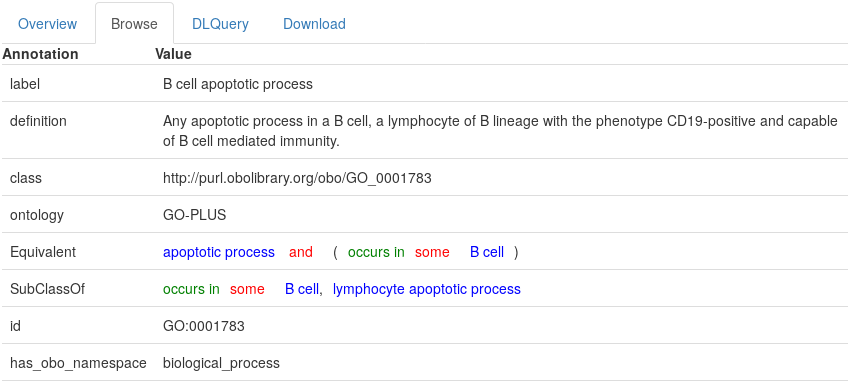
\includegraphics[width=1\textwidth]{bcellapoptosis.png}
\end{frame}

\begin{frame}
  \frametitle{Ontologies: axioms, not graphs!}
  Gene Ontology:
  \begin{itemize}
  \item {\tt behavior DisjointWith: 'developmental process'}
  \item {\tt behavior SubclassOf: only-in-taxon some metazoa}
  \item {\tt 'cell proliferation' DisjointWith: in-taxon some fungi}
  \item {\tt 'cell growth' EquivalentTo: growth and ('results in
      growth of' some cell)}
  \item ...
  \end{itemize}
\end{frame}

% \begin{frame}
%   \frametitle{Ontologies: axioms, not graphs!}
%   \begin{itemize}
%   \item converting ontologies to graphs
%     \begin{itemize}
%     \item loses information
%     \end{itemize}
%   \item relations between ontologies
%   \end{itemize}
% \end{frame}

\begin{frame}
  \frametitle{Ontology embeddings}
  \begin{definition}
    Let $O = (\Sigma = (C, R, I); ax; \vdash)$ be an ontology with a set of
    classes $C$, a set of relations $R$, a set of instances $I$, a set
    of axioms $ax$ and an inference relation $\vdash$. An ontology
    embedding is a function $f_\eta : C \cup R \cup I \mapsto
    \Re^n$ (or $\Sigma(O) \mapsto \Re^n$. % (subject to certain constraints).
  \end{definition}
  \pause For example, we can use co-occurrence within $ax^\vdash$ to
  constrain the embedding function, where the constraints on
  co-occurrence are formulated using the Word2Vec skipgram model.
\end{frame}

\begin{frame}
  \frametitle{Onto2Vec}
  \centerline{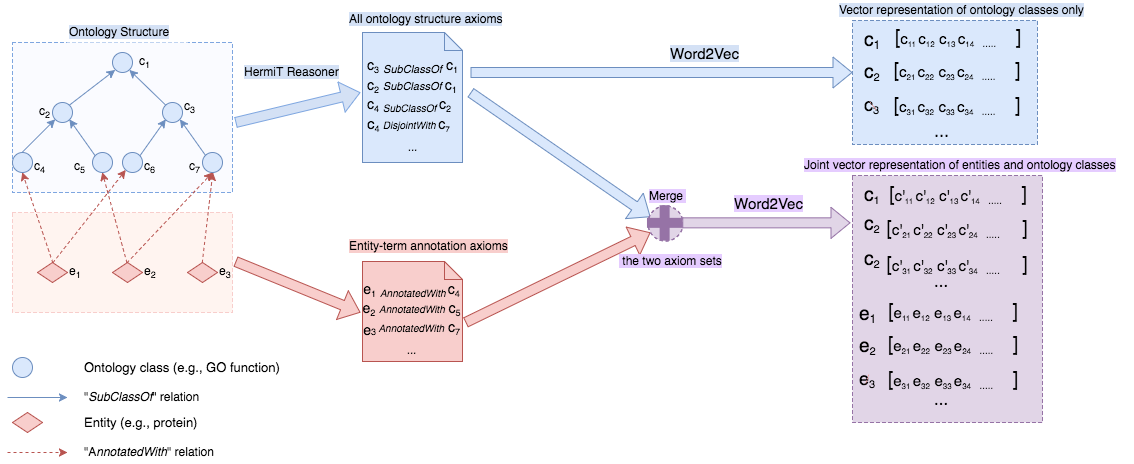
\includegraphics[width=\textwidth]{onto2vecflow.png}}
\end{frame}

\begin{frame}
  \frametitle{Word2Vec}
  Maximize:
  \begin{equation}
    \frac{1}{N} \sum_{n=1}^{N} \sum_{-c\leq j \leq c, j\not=
      0} \log p(w_{n+j}|w_n)
  \end{equation}
  with
  \begin{equation}
    p(w_o | w_i) = \frac{\exp({v'_{w_o}}^T v_{w_i})}{\sum_{w=1}^{W}
      \exp({v'_{w}}^T v_{w_i})}
  \end{equation}
  (at least conceptually; different strategies are used to approximate Eqn. 2)
\end{frame}

\begin{frame}
  \frametitle{Word2Vec}
  \centerline{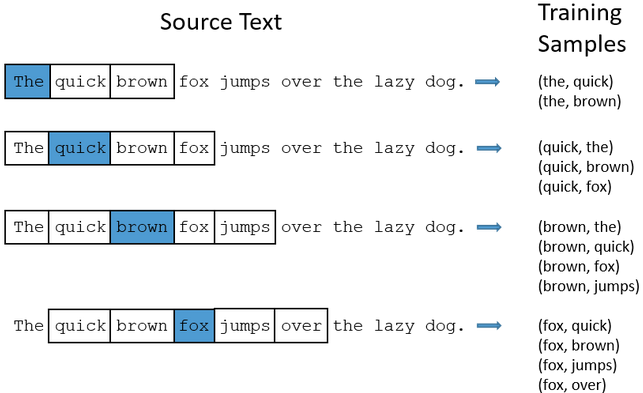
\includegraphics[width=\textwidth]{word2vec-example.png}}
\end{frame}

\begin{frame}
  \frametitle{Predicting PPIs: trainable similarity measures}
  \centerline{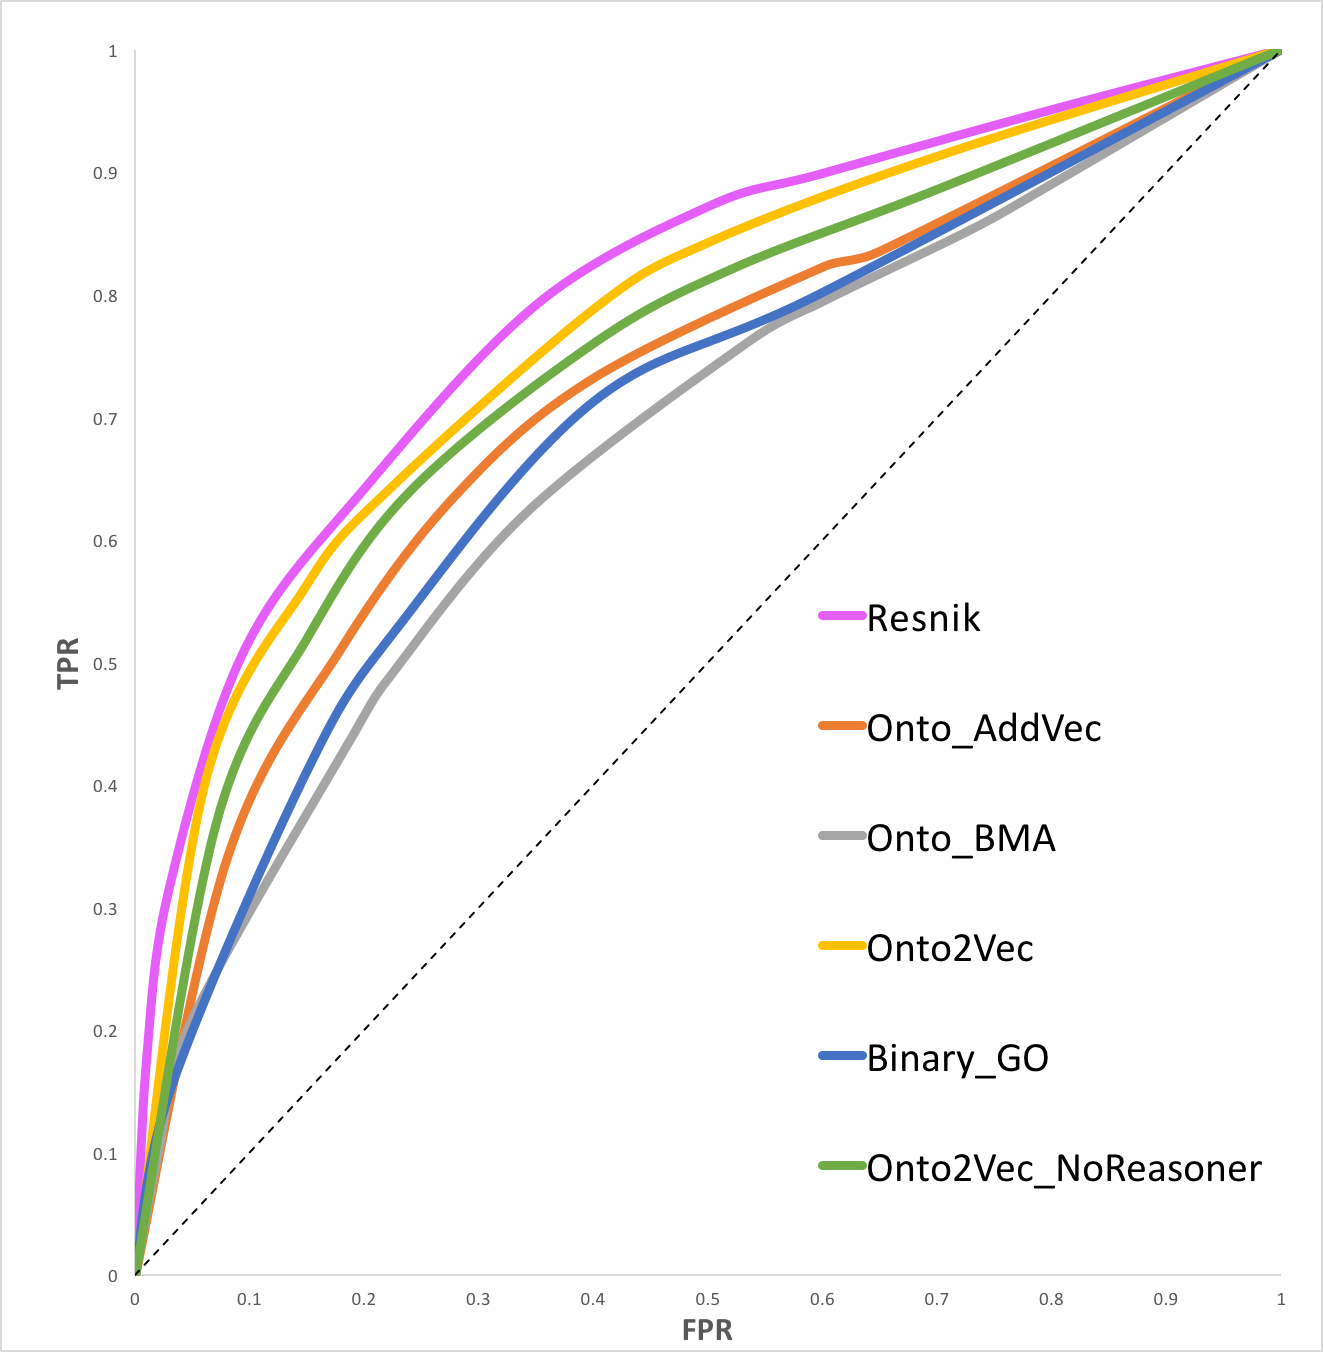
\includegraphics[width=.45\textwidth]{YSTUnsuper1.png}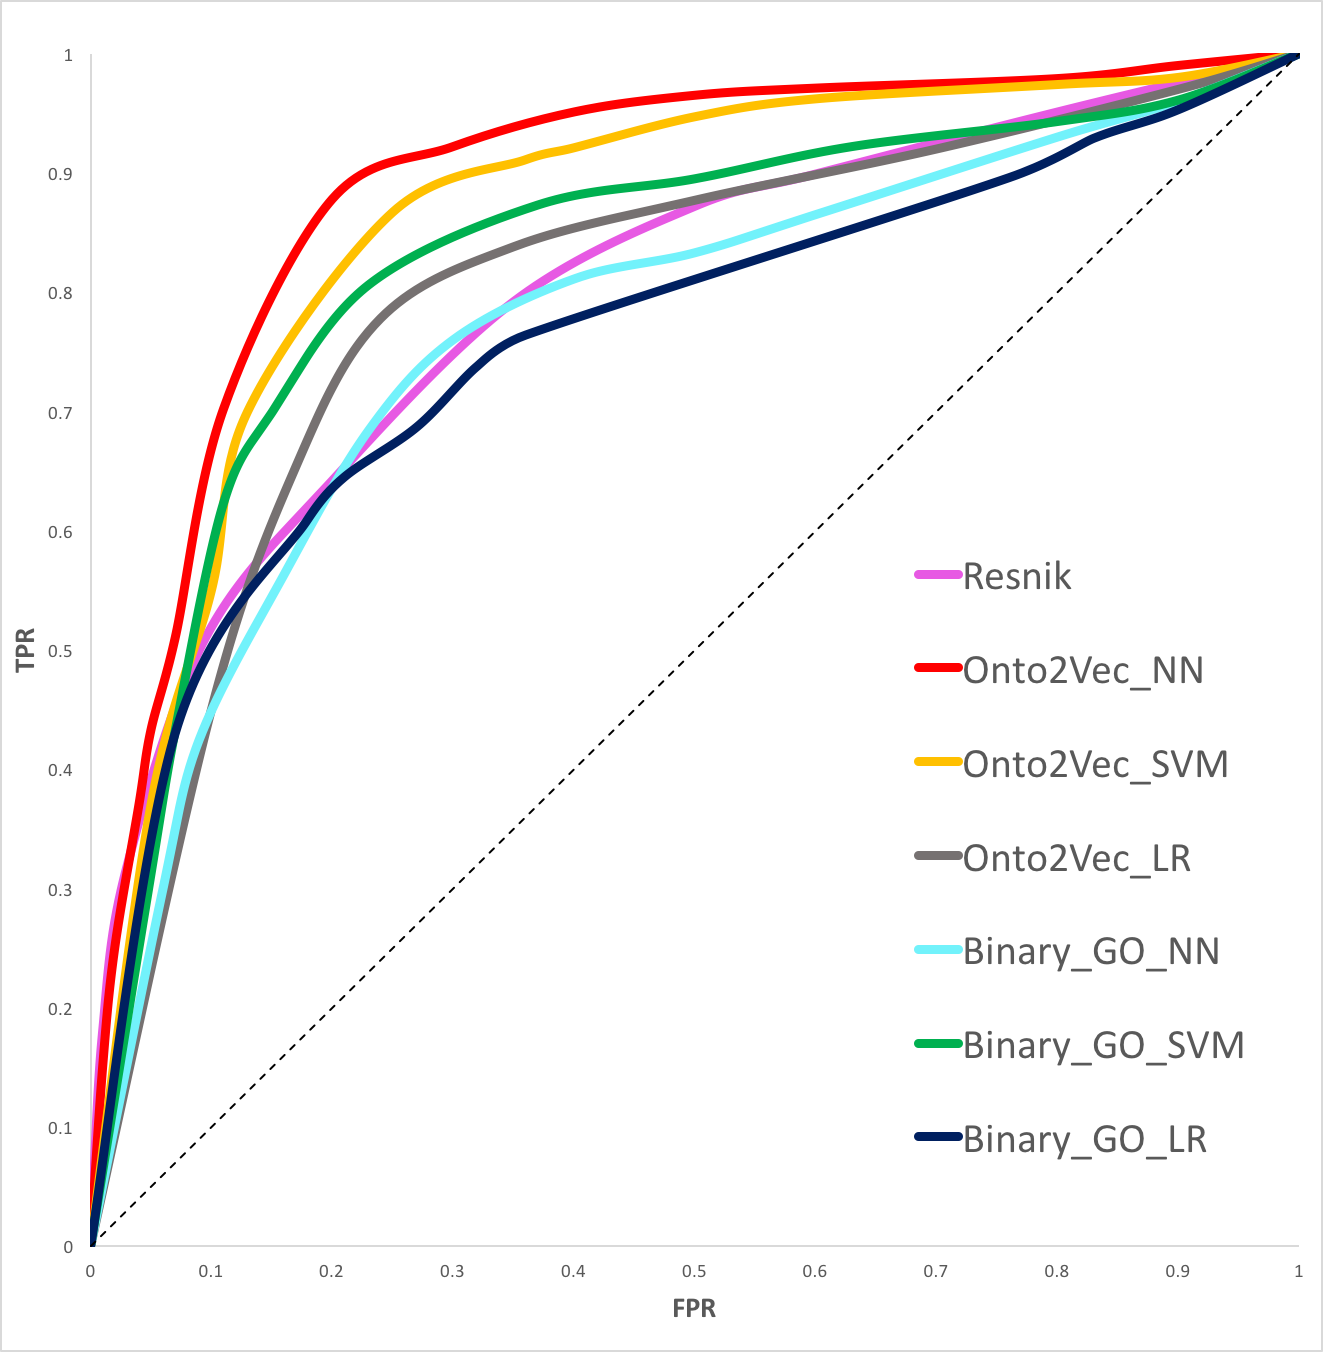
\includegraphics[width=.45\textwidth]{YstUnsup2.png}}

   {\tiny Smaili et al. Onto2Vec: joint vector-based representation of
     biological entities and their ontology-based annotations.}
\end{frame}

\begin{frame}
  \frametitle{Visualizing embeddings}
  \centerline{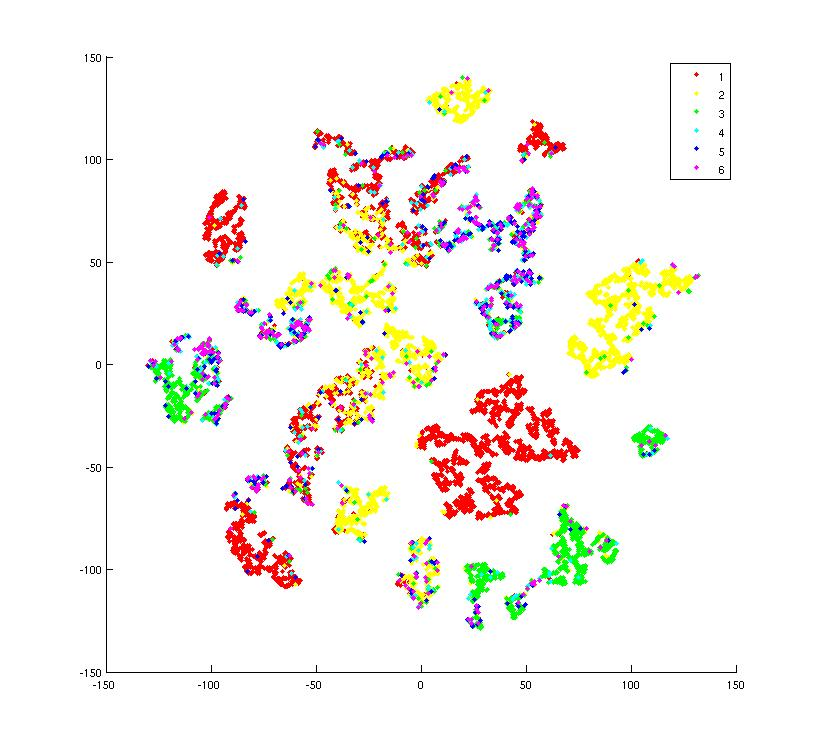
\includegraphics[width=.9\textwidth]{updtsne.jpg}}
\end{frame}

\begin{frame}
  \frametitle{Combination with text}
  \begin{itemize}
  \item ontologies contain more than axioms:
    \begin{itemize}
    \item labels, synonyms, definitions, authors, etc.
    \end{itemize}
  \item Description Logic axioms != natural language
  \item transfer learning: learn on one domain/task, apply to another
    \begin{itemize}
    \item e.g.: learn on literature, apply to ontologies
    \item words have ``meaning'' in literature, Description Logic
      symbols have ``meaning'' in ontology axioms
    \end{itemize}
  \item Ontologies Plus Annotations 2 Vec (OPA2Vec) combines both
  \end{itemize}
\end{frame}

\begin{frame}
  \frametitle{Ontologies Plus Annotations 2 Vec}
  \centerline{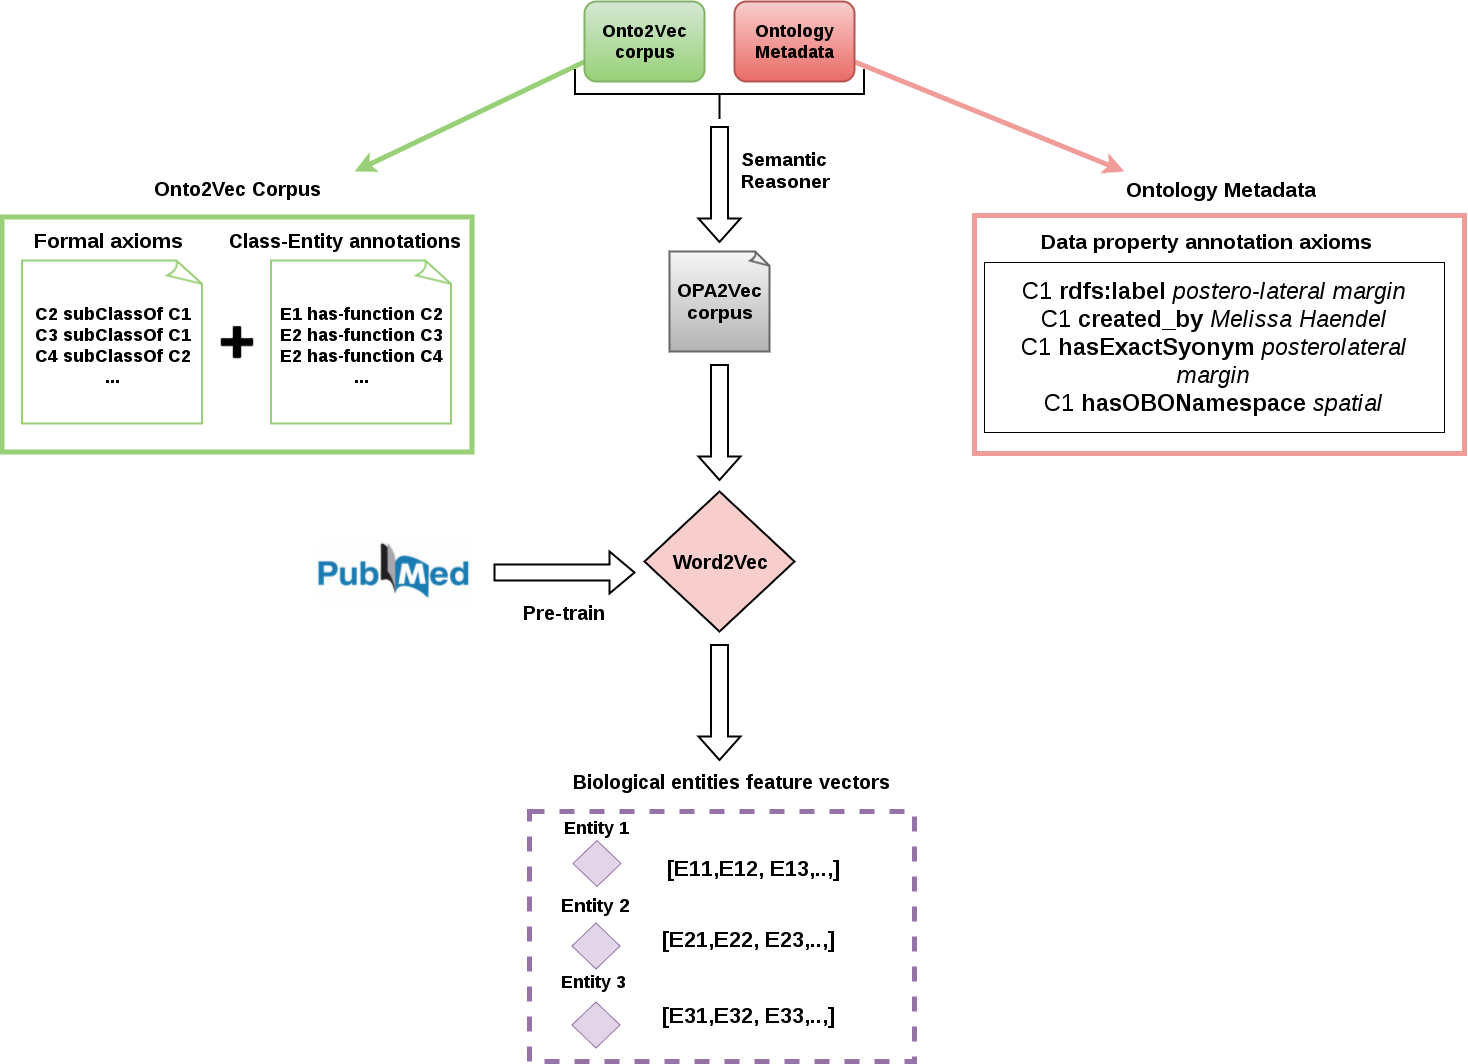
\includegraphics[width=1\textwidth]{opaworkflow16.png}}
\end{frame}

\begin{frame}
  \frametitle{Axioms contribute to prediction tasks: GO and GO-PLUS}
    % \processtable
    % \caption{AUC values of ROC curves for PPI prediction for
    %   GO-Plus and GO using Onto2Vec (cosine similiarity) and
    %   Onto2Vec-NN (neural network).\label{Tab:GOplus}}
    { \begin{tabularx}{\columnwidth}{XXXXXXX}\toprule & {}& {} &
                                                                 Human & Yeast & Arabidopsis\\\midrule
        $GO\_Onto2Vec$ & {} &{}& 0.7660 & 0.7701 & 0.7559 \\
        $GO\_Onto2Vec\_NN$ & {} & {}& 0.8779& 0.8711 & 0.8364 \\
        $GO\_plus\_Onto2Vec$ & {} & {}& 0.7880& 0.7943 & 0.7889 \\
        $GO\_plus\_Onto2Vec\_NN$ &{} & {}& \textbf{0.9021}&\textbf{0.8937} & \textbf{0.8834}\\
        \hline
      \end{tabularx}}{}
\end{frame}

\begin{frame}
  \frametitle{Evaluating individual axioms}
%  Testing how much each ontologies' axioms contribute to predictions:
%  \begin{resizebox}{\textwidth}{!}{
  Testing how much each ontologies' axioms contribute to predictions:
  \tiny
      \begin{tabularx}{\linewidth}{X|XX|XX}
        \toprule
        {} & \multicolumn{2}{c}{\textbf{Human}} & \multicolumn{2}{c}{\textbf{Arabidopsis}}\\
        \midrule
        {} & \textbf{Onto2Vec}&\textbf{Onto2Vec\_NN} &\textbf{Onto2Vec}&\textbf{Onto2Vec\_NN} \\
        \midrule
        GO (Baseline) &0.7660 &0.8779  & 0.7559 & 0.8364 \\
        ChEBI &0.7899\textcolor{blue}{(+0.0239)}& 0.8914\textcolor{blue}{(+0.0135)}  & 0.7703\textcolor{blue}{(+0.0144)}& 0.8518\textcolor{blue}{(+0.0154)} \\
        PO &0.7752\textcolor{blue}{(+0.0092)} & 0.8776\textcolor{red}{(-0.0003)} & 0.7671\textcolor{blue}{(+0.0112)} & 0.8469\textcolor{blue}{(+0.0105)}\\
        CL & 0.7743\textcolor{blue}{(+0.0083)} & 0.8810\textcolor{blue}{(+0.0031)} & 0.7612\textcolor{blue}{(+0.0053)}& 0.8371\textcolor{blue}{(+0.0007)}\\
        PATO & 0.7657\textcolor{red}{(-0.0003)} & 0.8768\textcolor{red}{(-0.0011)} & 0.7563\textcolor{blue}{(+0.0004)} & 0.8380\textcolor{blue}{(+0.0016)}\\
      \end{tabularx}
%    }
%  \centerline{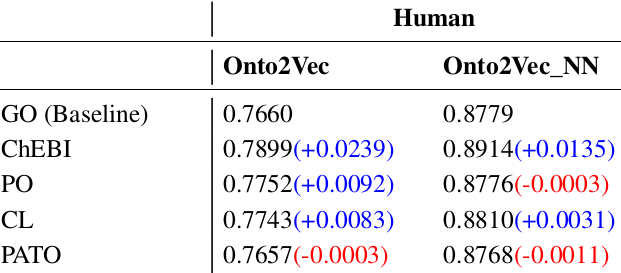
\includegraphics[width=1\textwidth]{pato-eval1.png}}
\end{frame}

\begin{frame}
  \frametitle{Evaluating definitions}
  Testing how much each ontologies' annotation properties contribute to predictions:
  \tiny
      \begin{tabularx}{\linewidth}{X|XX|XX}
        \toprule
        {} & \multicolumn{2}{c}{\textbf{Human}} & \multicolumn{2}{c}{\textbf{Arabidopsis}}\\
        \midrule
        {} & \textbf{Onto2Vec}&\textbf{Onto2Vec\_NN} &\textbf{Onto2Vec}&\textbf{Onto2Vec\_NN} \\
        \midrule
        GO (Baseline)&0.8727 &0.9033  & 0.8613 & 0.8903 \\
        ChEBI & 0.8571\textcolor{red}{(-0.0156)} &0.8801\textcolor{red}{(-0.0232)} &0.8601\textcolor{red}{(-0.0012)}& 0.8880\textcolor{red}{(-0.0023)}\\
        PO & 0.8680\textcolor{red}{(-0.0047)}&0.8824\textcolor{red}{(-0.0209)} & 0.8632\textcolor{blue}{(+0.0019)} & 0.8908\textcolor{blue}{(+0.0005)}\\
        CL & 0.8811\textcolor{blue}{(+0.0084)}&0.9037\textcolor{blue}{(+0.0004)}  & 0.8614\textcolor{blue}{(+0.0001)} & 0.8899\textcolor{red}{(-0.0004)}\\
        PATO & 0.8562\textcolor{red}{(-0.0165)}& 0.8711\textcolor{red}{(-0.0322)} & 0.8544\textcolor{red}{(-0.0069)}& 0.8860\textcolor{red}{(-0.0043)} \\
      \end{tabularx}
%  \centerline{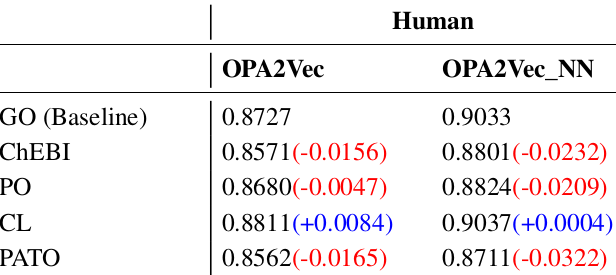
\includegraphics[width=1\textwidth]{pato-eval2.png}}
\end{frame}

\begin{frame}
  \frametitle{OPA2Vec}
  \begin{itemize}
  \item \url{https://github.com/bio-ontology-research-group/opa2vec}
  \item command line tool
    \begin{itemize}
    \item input: OWL ontology, set of entities with annotations/associations
    \item output: vectors for each class and entity
    \end{itemize}
  \item includes Elk and HermiT
  \item limitations: word-based
    \begin{itemize}
    \item completely ignores any semantics!
    \end{itemize}
  \end{itemize}
\end{frame}

\begin{frame}
  \frametitle{More}
  \url{https://github.com/bio-ontology-research-group/ontology-tutorial}
  \begin{itemize}
  \item more slides
    \begin{itemize}
    \item ontology theory
    \item machine learning
    \item applications
    \end{itemize}
  \item code examples, executable notebooks, all dockerized!
    \begin{itemize}
    \item predict gene--disease associations through phenotype similarity
    \item protein--protein interactions
    \end{itemize}
  \end{itemize}
\end{frame}

\end{document}
%%% Local Variables:
%%% mode: latex
%%% TeX-master: t
%%% End:
